\documentclass[letterpaper,12pt]{article}
\usepackage[utf8]{inputenc}
\usepackage{charter}
\usepackage{geometry}
\usepackage{amsmath}
\usepackage{float}
\usepackage{graphicx}
\usepackage{subcaption}
\usepackage{amssymb}
\usepackage{adjustbox}
\usepackage{wrapfig} 
\usepackage{xcolor}
\usepackage{fancyhdr}
\usepackage{tabularx}
\usepackage{fancyhdr}
\usepackage{comment}

\geometry{top=2cm, bottom=2cm, left=2cm, right= 2cm} %%margen
\graphicspath{{images/}}
\parindent=0pt

\begin{document}
%%para contador y eso
\thispagestyle{empty}
\newpage
\setcounter{page}{1}
\pagestyle{headings}
%%%%%%%%%%%%%%%%%%%%%%%%%%%%%%%%%%%%%%%%%%%%%%%%%%%%%%%%%%%%%%%%%%%%%%%%%%%%
\begin{sloppypar} 
    %%%portadita
    \begin{titlepage}
        \fancyhead{R}{
        
\includegraphics[width=0.1\linewidth]{logoUV.png}
        }
        \hspace{2.5cm}
        {\bfseries\LARGE Universidad Veracruzana \par}
        \hspace{2cm}
        {\scshape\Large Facultad de Ingeniería Eléctrica y Electrónica \par}
        \begin{center}
            \vspace{7cm}
            {\itshape\huge Bases de Datos \par}
            {\itshape\Large Práctica 1 \par}
            {\large Lara Xocuis Martha Denisse\par}
            {\large S22002213 \par}
            \vfill
            {\Large September 2, 2024 \par}
        \end{center}
    \end{titlepage} 

%%%%%%%%%%%%%%%%%%%%%%INFO%%%%%%%%%%%%%%%%%%%%%%
\textbf{ACTIVIDADES:}
\section*{Leer el capítulo 1 del libro: "FUNDAMENTOS DE BASES DE DATOS" de Abraham Silberschatz}
\begin{itemize}
    \item \textbf{¿Cuál es el propósito de los sistemas de bases de datos?} \\ Uno de los propósitos principales de los sistemas de bases de datos es ofrecer a los usuarios una visión abstracta de los datos. Es decir, buscan acabar con la redundancia e inconsistencia de los datos, dificultad, aislamiento, problemas de integridad y seguridad.
    \item \textbf{¿Cuáles son las desventajas del sistema de procesamiento de archivos?} \\ Dependencia de datos del programa, duplicación de datos, compartir datos de forma limitada, tiempos de desarrollo largos y mantenimiento excesivo del programa.
    \item \textbf{Analice con detalle los tres niveles de abstracción de datos}
    \begin{enumerate}
        \item Nivel \textbf{FÍSICO}: Describe \textbf{\textit{cómo}} se almacenan realmente los datos.
        \item Nivel \textbf{LÓGICO}: Describe \textbf{\textit{qué}} datos se almacenan en la base de datos y que relaciones existen entre esos datos.
        \item Nivel \textbf{VISTA}: Simplifica su \textbf{interacción} con el sistema.
    \end{enumerate}
    \item \textbf{Revisar la sección 1.11 Arquitectura de las bases de datos} \\ 
    La arquitectura de los sistemas de bases de datos puede variar considerablemente según el entorno en el que se implementen. Existen diferentes tipos de arquitecturas:
    \begin{itemize}
        \item \textbf{Centralizadas}: Donde la base de datos se gestiona desde un único sistema central.
        \item \textbf{Cliente-servidor}: En esta configuración, una máquina servidora maneja las solicitudes de múltiples clientes.
        \item \textbf{Paralelas}: Aprovechan la computación paralela para procesar consultas y datos de manera eficiente.
        \item \textbf{Distribuidas}: Se extienden a través de múltiples máquinas localizadas en distintas ubicaciones geográficas.
    \end{itemize}

    \item \textbf{Analice con detalle la figura 1.7 Arquitecturas de dos y tres capas. }\\ \textit{\underline{Arquitectura de dos capas:}} La aplicación se divide en un componente cliente, que se comunica directamente con el servidor de bases de datos a través de lenguajes de consulta como SQL, utilizando estándares como ODBC y JDBC. 
    \vspace{0.3cm}\\ 
    \textit{\underline{Arquitectura de tres capas:}} El cliente actúa solo como interfaz para el usuario. La comunicación entre el cliente y el servidor de bases de datos se realiza a través de un servidor de aplicaciones que gestiona la lógica de negocio y las interacciones con la base de datos. Esta arquitectura es adecuada para aplicaciones grandes y en la web.
    \newpage
    \item \textbf{Leer la sección 1.12.1 Usuarios de bases de datos e interfaces de usuario.}
    \begin{itemize}
        \item \textbf{Usuarios normales}: Usuarios no sofisticados que interactuan con el sistema invocando alguno de los programas de aplicación que se han escrito previamente.
        \item \textbf{Programadores de aplicaciones}: profesionales informáticos que escriben programas de aplicación.
        \item \textbf{Usuarios sofisticados}: interactuan con el sistema sin escribir programas, formulan sus consultas en un lenguaje de consultas de bases de datos.
        \item \textbf{Usuarios especializados}: escriben aplicaciones de bases de datos especializadas que no encajan en el marco tradicional del procesamiento de datos.
    \end{itemize}


    \item \textbf{Estudiar la sección 1.13 Historia de los sistemas de bases de datos:} 
    \begin{enumerate}
        \item Principios del siglo XX: Las tarjetas perforadas, inventadas por Herman Hollerith, se usaron para el censo de EE.UU. y se introdujeron en las computadoras para registrar datos.
        \item Década de 1950 y principios de 1960: Se desarrollaron cintas magnéticas para almacenar datos, permitiendo la automatización de tareas como la elaboración de nóminas.
        \item Finales de los años 60 y 70: La introducción de discos duros permitió el acceso directo a los datos, liberando el procesamiento de la secuencialidad. 
        \item Años 80: A pesar de la complejidad inicial, las bases de datos relacionales superaron a las de red y jerárquicas en rendimiento y facilidad de uso, gracias a proyectos como System R de IBM
        \item Principios de los años 90: Se enfatizó en el uso de SQL para aplicaciones intensivas en consultas y análisis de datos.
        \item Principios del siglo XXI: Se introdujo XML y su lenguaje de consulta, XQuery, en las bases de datos. 
    \end{enumerate}
    \newpage
    \item \textbf{Responder de la sección de Ejercicios prácticos}
    \begin{itemize}
        \item 1.1 En este capítulo se han descrito varias ventajas importantes de los sistemas gestores de bases de datos. ¿Cuáles son sus dos inconvenientes?
        \begin{itemize}
            \item Los costos y mantenimiento de dicho gestor; son muy elevados los costos y retos que debe pasar una empresa (como ejemplo) si quiere prevalecer con un buen gestor.
        \end{itemize}
        \item 1.2 Indíquese siete lenguajes de programación que sean procedimentales y dos que no lo sean. ¿Qué grupo es más fácil de aprender a usar? Explíquese la respuesta.
        \begin{itemize}
            \item \textit{Procedimentales}: C, Pascal, Fortran, BASIC, ada, Modula-2, COBOL; Dos que no lo son serían JavaScript y Prolog. \\ Los procedimentales son más fáciles de aprender ya que tienen una estructura y lógica clara, los otros tenemos la necesidad de una comprensión más profunda.
        \end{itemize}
        \item 1.5 Indíquese cuatro aplicaciones que se haya usado que sea muy posible que utilicen un sistema de bases de datos para almacenar datos persistentes.
        \begin{itemize}
            \item He utilizado apps como Bancomer, Instragram, Youtube y Notion.
        \end{itemize} 
        \item 1.6 Indíquense cuatro diferencias significativas entre un sistema de procesamiento de archivos y un SGBD.
        \begin{itemize}
            \item El sistema de procesamiento de archivos duplica datos por su redundancia, los datos dependen den otros programas, son locales y puede alterar la calidad de dichos datos, cosa que un SGBD evita a toda costa.
        \end{itemize}
        \item 1.7 Explíquese la diferencia entre independencia de datos física y lógica. 
        \begin{itemize}
            \item Independencia física es cambiar cosas de dónde estan guardados los datos (aplicaciones o almacenamiento) sin afectar su contenido y la lógica es la parte contraria, cambiar la información de los datos o diseño sin afectar su almacenamiento físico.
        \end{itemize}
    \end{itemize}
\end{itemize}
\newpage
%%%%%%%%%%%%%%%%%%%%%%%%%%%%%%%%%%%%%555
\section*{Leer la Parte 1 del libro: "MODERN DATABASE MANAGEMENT" de Jeffrey A. Hoffer: "The Context of Database Management"}
\begin{itemize}
    \item \textbf{Lea con cuidado la sección "BASIC CONCEPTS AND DEFINITIONS" }
    \begin{itemize}
        \item \textbf{Note la diferencia entre dato e información}
        \begin{center}
                \begin{tabular}[H]{|c|c|} \hline 
                \textbf{DATO} & \textbf{INFORMACIÓN} \\ \hline  
                - Representación almacenada de & - Datos que han sido procesados\\
                objetos y eventos & que permiten que el conocimiento \\
                que tienen un significado & del usuario incremente \\
                importante para el usuario & \\ \hline
                \end{tabular}   
        \end{center}

        \item \textbf{Ponga especial énfasis en “Metadatos”} \\ Comúnmente es conocido como "\textit{datos de datos}", describe las \textbf{características} de los datos. 
        \item \textbf{¿Cuáles son las desventajas del sistema de procesamiento de archivos?}
        \begin{itemize}
            \item \textbf{Duplicación} de datos
            \item \textbf{Dependencia} de programas.
            \item Compartir datos de forma \textbf{limitada}
            \item \textbf{Tiempo extenso} de desarrollo
            \item \textbf{Mantenimiento excesivo} del programa
        \end{itemize}
        \item \textbf{Analice la definición de este autor para un SGBD} \\ Un Sistema Gestor de Base de Datos es un software que es usado para crear, manipular y controlar el acceso a los usuarios a una base de datos. Provee un método sistemático para \textbf{crear, actualizar y almacenar datos} guardados en una BD.
        \item \textbf{¿Cuáles son las ventajas/desventajas de la propuesta de bases de datos?}
        \begin{center}
            \begin{tabular}[H]{|c|c|} \hline
            \textbf{VENTAJAS} & \textbf{DESVENTAJAS} \\ \hline
            - Independencia hacia un programa & -Personal nuevo y especializado\\ \hline 
            - Redundancia mínima & -Instalación y mantenimiento costoso\\ \hline
            - Mejora la consistencia de los datos & -Necesidad por copias de respaldo explicitas \\ \hline
            - Mejora la accesibilidad de datos & - Conflicto empresarial \\ \hline
            - Mejora la calidad de datos & \\ \hline
                
            \end{tabular}
        \end{center}

        \item \textbf{¿Qué es una restricción?}\\ Una regla que no puede ser violada por el usuario de la base de datos
        \item \textbf{¿Cuáles son los costos y riesgos de utilizar BD?}
        \begin{itemize}
            \item Personal nuevo y especializado
            \item Instalación y mantenimiento costoso
            \item Necesidad por copias de respaldo explícitas
            \item Conflicto empresarial
        \end{itemize}
        \newpage
        \item \textbf{¿Cuáles son los componentes del ambiente de BD?}
        \begin{itemize}
            \item CASE TOOLS: Software de ingeniería.
            \item Repositorios: almacenamiento de \textbf{metadatos} centralizados
            \item Base de datos: almacén de datos
            \item Programas: software que usan los datos
            \item Interfaz de usuario: pantalla textual y gráfica para los usuarios.
            \item Administrador de datos: personal responsable para el manejo de una base de datos
            \item Desarolladores de sistemas
            \item Programadores: personal responsable para diseñar una base de datos y software
            \item "END-USERS": personas quienes usan las aplicaciones
        \end{itemize}
        \item \textbf{Analice el ambiente de aplicación de las BD de dos y tres capas}  
        \begin{itemize}
            \item \textbf{Dos capas:} servidor de dos clientes, son útiles cuando una BD personal debe ser compartida entre varios usuarios. Funciona como una red local.
            \item \textbf{Tres o múltiples capas:} abordan las limitaciones de las de dos capas, divide la aplicación en varias capas, esto es común en aplicaciones modernas diseñadas para soportar un gran número de usuarios.
        \end{itemize}
        \item \textbf{¿Qué es un ERP?} \\ Sistema de gestión empresarial que integra todas las funciones de una empresa; como fabricación, ventas, finanzas, marketing, inventario, contabilidad y recursos humanos. Estos también son aplicaciones que proporcionan los datos necesarios a la empresa para examinar y gestionar sus actividades.
    \end{itemize}
    \item \textbf{Revise la sección correspondiente a la evolución de los sistemas de BD} \\ El sistema gestor de base de datos surgieron en la década de los 60 y han evolucionado desde entonces. Esta ha sido impulsada por cuatro objetivos principales:
    \begin{enumerate}
        \item Independencia entre programas
        \item Gestión de datos complejos
        \item Acceso fácil a los datos
        \item Plataformas para soporte a la toma de decisiones
    \end{enumerate}
    A continuación se hacen menciones importantes entre cada decada y evolución de los sistemas de bases de datos:

    \begin{itemize}
        \item 60s: los sistemas de archivos dominaban en esta época, se introdujeron los primeros sistemas de gestión de bases de datos (SGBD). Este período se considera un "prueba de concepto" para demostrar la viabilidad de gestionar grandes volúmenes de datos con un SGBD.
        \item 70s: Ya existia de forma comercial los SGBD, se desarrollaron los modelos jerárquico y de red para manejar estructuras de datos más complejas, estos sufrieron de desventajas clave como la limitada independencia de los datos y largos tiempos de desarrollo para las aplicaciones.
        \item 80s: Ed Codd desarrolló el sistema de modelo de datos relacional, este modelo representa todos los datos en forma de tablas y usa SQL para la recuperación de datos.
        \item 90s: Marcó el inicio de la era de la informática cliente/servidor, el almacenamiento de datos y las aplicaciones en Internet. Los datos gestionados por los SGBD se expandieron a datos multimedia.
        \item 2000 en adelante: Los SGBD relacionales siguen siendo los más utilizados, pero los orientados a objetos están ganando atención.
    \end{itemize}


    \item \textbf{Revisar el ciclo de vida de desarrollo de sistemas, que también aplica a las BD} \\ El ciclo de vida de desarollo de sistemas, por su definición, la metodología tradicional usada para desarollar, mantener, y sustituir sistemas de información. Es un completo set de pasos para diseñadores de bases de datos.
    \begin{itemize}
        \item Planificación
        \item Análisis
        \item Diseño
        \item Implementación
        \item Mantenimiento
    \end{itemize} 
    
    \item \textbf{Analizar con detalle el resumen del capitulo} \\
    \textbf{Una base de datos} es una colección organizada de datos lógicamente almacenados donde, los datos son representaciones almacenadas de objetos relevantes para el usuario.
    \vspace{0.3cm}\\ 
    \textbf{La información, }por su parte, se refiere a datos procesados que aumentan el conocimiento del usuario. Los metadatos son datos que describen características de los datos.
    \vspace{0.3cm}\\ 
    \textbf{Un sistema gestor de base de datos (SGBD)} es un software que crea, mantiene y controla el acceso a las bases de datos, este almacena metadatos en un repositorio central.
    \vspace{0.3cm}\\ 
    \textbf{Los sistemas de procesamiento de archivos }presentan varias limitaciones como: dependencia de datos hacia programas, duplicación de datos y tiempos largos de desarollo/mantenimiento. Los SGBD se desarrollaron para superar estas limitaciones.
    \vspace{0.3cm}\\ 
    \textbf{Las aplicaciones de bases de datos} se dividen en: personales  (dos niveles) múltiples capas y empresariales (para las ERP).
    \newpage
    \item \textbf{Realizar los ejercicios de la página 44 hasta la pregunta 12}
    
    \begin{enumerate}
        \item \textbf{Define cada termino a continuación:} 
        \begin{itemize}
            \item \textbf{dato:} representación almacenada de objetos y eventos que tienen un significado e importancia al usuario.
            \item \textbf{información:} datos que han sido procesados de tal modo que el conocimiento del usuario incremente.
            \item \textbf{metadato:} datos que describen las propiedades o características de los datos.
            \item \textbf{aplicación de base de datos:} programa de aplicación (o conjunto de programas relacionados) que se utilizan para realizar actividades de base de datos en nombre de los usuarios.
            \item \textbf{almacén de datos:} base de datos integrada de apoyo cuyo contenido se deriva
            de las distintas bases de datos
            operativas.
            \item \textbf{restricción: }una regla que no puede ser violada por el usuario de la base de datos
            \item \textbf{base de datos:} colección organizada de datos
            lógicamente relacionados.
            \item \textbf{entidad: }una persona, un lugar, un objeto, un evento o un concepto en el ambiente del usuario acerca de cual organización desea manejar esos datos.
            \item \textbf{sistema gestor de base de datos:} un software que es usado para crear, gestionar y proporcionar control de acceso a las bases de datos de los usuarios.
            \item \textbf{arquitectura cliente/servidor:} modelo informático en red que distribuye los procesos entre clientes y servidores, que suministran
            los servicios solicitados. 
            \item \textbf{ciclo de vida de desarollo de sistemas: }metodología tradicional utilizada para desarrollar, mantener y sustituir sistemas de información.
            \item \textbf{desarollo ágil de software:} enfoque del desarrollo de bases de datos y desarrollo de software que se enfoca en: "el software de trabajo
            documentación exhaustiva, la colaboración con el cliente negociación de contratos"
            \item \textbf{modelo de datos empresariales:} el primer paso en el desarrollo desarrollo de bases de datos, en el que y el contenido general de bases de datos organizativas se especifican datos
            \item \textbf{modelo de datos conceptuales: }una especificación detallada independiente de la tecnología estructura general de los datos
            \item \textbf{modelo de datos lógicos: }representación de una base de datos por una particular tecnología de gestión de datos 
            \item \textbf{modelo de datos físicos:} especificaciones sobre cómo se almacenan los datos de un esquema lógico se almacenan en memoria secundaria de un ordenador un sistema de gestión de bases de datos.
        \end{itemize}
        \newpage
        \item \textbf{Empareja los siguientes términos y definiciones}
        \begin{center}
            \begin{tabular}[H]{|c|c|} \hline
            \textit{\textbf{\large término}} & \textit{\textbf{\large definición}} \\ \hline 
            dato (c) & hechos, texto, gráficas, etc\\ \hline
            
            aplicación de base de datos (b) & programa de aplicación\\ \hline

            restricción (l) & una regla que no puede ser \\ 
            & violada por los usuarios de \\ 
            & base de datos \\ \hline

            repositorio(g) & almacén centralizado de las\\ 
            & definiciones de los datos \\ \hline

            metadato(f) & incluye definiciones de datos\\
            & y restricciones \\ \hline

            almacén de datos(m) & base de datos de soporte \\ 
            & para la toma de decisiones \\\hline
            
            información(a) & datos en contexto o resumidos\\ \hline
            
            vista de usuario(j) & descripción lógica de una parte\\
            & de la base de datos \\\hline
            
            SGBD (k) & un software que se usa para \\ 
            & crear, gestionar y proporcionar\\ 
            & control a una base de datos \\ \hline
            
            independencia de datos (h) & separación de descripciones de \\
            & datos a los programas \\ \hline
            
            planificación de recursos empresariales(i) & sistema de gestión empresarial que \\ 
            & integra funciones de la empresa\\ \hline
            
            ciclo de vida de desarollo de sistemas(r) & enfoque estructurado, paso a paso\\
            & para el desarollo de sistemas\\ \hline
            
            creación de prototipos(o) & enfoque rápido para el \\
            & desarollo de sistemas\\ \hline
            
            modelo de datos empresariales(d) & modelo gráfico que muestra entidades\\
            & de alto nivel para la organización\\ \hline
            
            esquema conceptual(p) & consta en dos modelos de datos\\
            & modelo lógico y físico\\\hline
            
            esquema interno(n) & modelo de datos de la empresa \\ \hline
            
            esquema externo(q) & descripción de los datos del negocio\\ \hline 
            \end{tabular}
        \end{center}
    \end{enumerate}
    \item \textbf{Contrasta los siguientes términos}
    \begin{itemize}
        \item \textbf{Dependencia e Independencia de datos}
        \begin{itemize}
            \item Dependencia de datos: datos que dependen de un programa y que, si se modifica tal programa o archivo, los datos pueden ser alterados
            \item Independencia de datos: mayor efectividad y gestion de datos ya que no necesitan de otro programa para ser abiertos
        \end{itemize}
        \item \textbf{Datos Estructurados y no Estructurados}
        \begin{itemize}
            \item Estructurados: tienen un formato definido 
            \item No estructurados: es como texto libre, no tiene una estructura lógica
        \end{itemize}
        \newpage
        \item \textbf{Información y dato}
        \begin{itemize}
            \item Información: datos que han sido procesados
            \item Datos: representación simbólica de objetos
        \end{itemize}
        \item \textbf{Base de dato y repositorio}
        \begin{itemize}
            \item Base de dato: colección organizada de datos 
            \item Repositorio: almacena metadatos
        \end{itemize}
        \item \textbf{Entidad y modelo de dato empresarial}
        \begin{itemize}
            \item Entidad: una persona, un lugar, un objeto, un evento o un concepto en el ambiente del usuario acerca de cual organización desea manejar esos datos.
            \item Dato empresarial: los datos se relacionan y son utilizados dentro de una organización, considerando entidades, relaciones y reglas de negocio.
        \end{itemize}
        \item \textbf{Almacén de datos y sistema PRE}
        \begin{itemize}
            \item Almacén de datos: sistema de almacenamiento de datos diseñado para la consulta y análisis de datos.
            \item Sistema PRE: generación de informes y análisis basado en datos preexistentes
        \end{itemize}
        \item \textbf{Base de datos de dos niveles y base de datos de varios niveles}
        \begin{itemize}
            \item BD DOS NIVELES: está compuesto por un cliente y un servidor
            \item BD VARIOS NIVELES: cada nivel tiene una base de datos que gestiona hacia un enfoque en específico
        \end{itemize}
        \item \textbf{Ciclo de vida de desarollo de sistemas y creación de prototipos}
        \begin{itemize}
            \item Ciclo de vida de BD: conjunto de fases que se siguen para la planificación hasta la gestión de un sistema.
            \item Creación de prototipos: desarrollo de v prototipos del sistema para validar ideas.
        \end{itemize}
        \item \textbf{Modelado de datos empresariales y Modelado de datos conceptual}
        \begin{itemize}
            \item Modelado de datos empresariales: datos específicos dentro del contenido general organizacional
            \item Modelado de datos conceptual: especificación detallada independiente de la tecnología estructura general de los datos
        \end{itemize}
        \item \textbf{Creación de prototipos y desarollo ágil de software}
        \begin{itemize}
            \item Creación de prototipos: desarrollar versiones tempranas del sistema para evaluar ideas 
            \item Desarollo ágil de software: metodología de desarrollo que enfatiza la entrega de un software funcional.
        \end{itemize}
    \end{itemize}
    \newpage
    \item \textbf{Enlista cinco desventajas de sistema de procesamiento de archivos}
    \begin{enumerate}
        \item Redundancia de datos
        \item Dependencia de datos a ciertos programas
        \item Mantenimiento del programa excesivo
        \item Compartir datos de forma ilimitada
        \item Tiempo extenso de desarollo
    \end{enumerate}
    \item \textbf{Enlista los nueve mayores componentes en un ambiente de sistema de base de datos}
    \begin{enumerate}
        \item CASE TOOLS
        \item Repositorios
        \item Base de datos
        \item Programas
        \item Interfaz de usuario
        \item Administrador de datos
        \item Desarolladores de sistemas
        \item Programadores
        \item END-USERS
    \end{enumerate}
    \item \textbf{¿Cómo son las relaciones entre las tablas expresadas en una base de datos relacional?} \\ Son relaciones que se establecen entre entidades que tienen un registro en común incluidos en un archivo, este se llama relación. 
    \item \textbf{¿Qué significa el término "independencia de datos" y por qué es una meta importante?} \\ La separación del metadata a las aplicaciones que usan los datos se llama independencia de datos; con el ambiente de base de datos, los metadatos están almacenados en una localización central llamada repositorio, esta propiedad de los sistemas de bases de datos permiten a los datos de las organizaciones el mejorar y gestionar sus datos sin cambiar nada de las aplicaciones que los gestionan.
    \newpage
    \item \textbf{Enlista 10 beneficios potenciales en una base de datos debajo del sistema convencional de archivos}
    \begin{itemize}
        \item Incrementa la productividad de desarollo de aplicaciones
        \item Mejora la transmisión de datos
        \item Mejora la consistencia de datos
        \item Independencia de datos hacia otros programas
        \item Mejora la calidad de los datos
        \item Reduce el mantenimiento de los datos
        \item Redundancia mínima
        \item Mejora la accesibilidad de datos
        \item Incremento de mejora con el soporte de datos
        \item Mayor gestión de almacenamiento
    \end{itemize}
    \item \textbf{Enlista los costos o riesgos asociados con el sistema de base de datos}
    \begin{itemize}
        \item Personal especializado
        \item Instalación y gestión costosa y compleja
        \item Conversión de costos
        \item Necesidad por copia de respaldo explícito y recuperación
        \item Conflicto organizacional
    \end{itemize}
    \item \textbf{Define la arquitectura de base de datos de tres niveles} \\ Divide el procesamiento de datos en tres capas distintas, cada una con responsabilidades específicas. Este enfoque se utiliza para superar las limitaciones de la arquitectura de dos niveles, la aplicación del cliente debe manejar tanto la interfaz de usuario como la lógica de negocios. \\ Mejora la escalabilidad, el rendimiento y la mantenibilidad de las aplicaciones.
    \item \textbf{En la arquitectura de base de datos de tres niveles, es posible que no haya ninguna base de datos en un nivel concreto? En caso de que no,¿por qué? en caso contrario escriba un ejemplo}\\ Depende del nivel ya que cada capa se encarga de ciertas cosas en específico, esto quiere decir que si no hay una BD en cierto nivel, podría haber cierto "desequilibrio" aunque, esta arquitectura fue justo en distribuir los datos de manera eficiente.
    \item \textbf{Nombre cinco fases del ciclo de vida de desarollo de sistemas tradicionales y explique el propósito y resultados de cada fase}
    \begin{enumerate}
        \item Planificación: establecer objetivos y planificar cómo se llevará a cabo el desarrollo del sistema. 
        \item Análisis de requisitos: identificar lo que el sistema debe hacer desde la perspectiva de los usuarios.
        \item Diseño: define el diseño de base de datos, la interfaz de usuario y los componentes del software.
        \item Implementación: integración de componentes y pruebas iniciales.
    \end{enumerate}
\newpage
\end{itemize}
\section*{Leer el capítulo 1 del libro: "FUNDAMENTOS DE BASES DE DATOS" de Martha Elena Millán}
\begin{itemize}
    \item Analizar con detalle la arquitectura ANSI-SPARC de un SMBD
    \vspace{0.3cm}\\
    La arquitectura ANSI-SPARC, una arquitectura de un SGBD se basa en tres niveles (externo, conceptual e interno). Trata de \textbf{separar la forma en la que los usuarios ven los datos, de los detalles de almacenamiento físico de los mismos}. \\ El principio de \textbf{INDEPENDENCIA DE DATOS} hace posible que el administrador de la base de datos cambie la estructura física de la base de datos a nivel interno sin que el nivel externo se afecte.
        \vspace{0.3cm}\\ 
        \textbf{El nivel físico} trata con los mecanismos de almacenamiento físico que el sistema operativo utiliza.
        \vspace{0.3cm}\\ 
        \textbf{El nivel interno} describe la forma en \textbf{cómo} los datos se almacenan en la base de datos.
        \vspace{0.3cm}\\ 
        \textbf{El nivel conceptual} corresponde a la \textbf{descripción de datos} y las relaciones entre estos.
        \vspace{0.3cm}\\ 
        \textbf{El nivel externo} representa cada una de las partes de la base de datos que es relevante para cada usuario.
        \vspace{0.3cm}\\ 
        \begin{center}
            
        \textit{A continuación, un gráfico que muestra parte de la arquitectura:}
        \end{center}

        \begin{figure}[H]
            \centering
            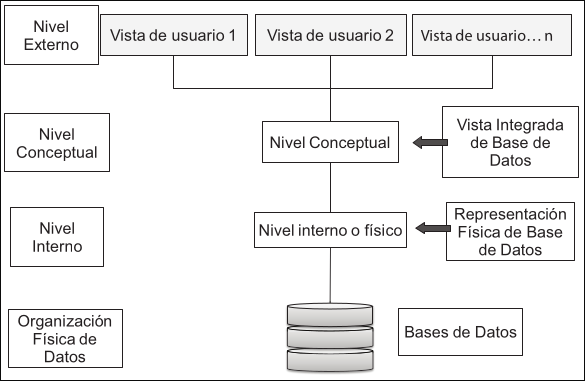
\includegraphics[width=0.8\textwidth]{ss.png}
            \caption{Arquitectura ANSI-SPARC}
        \end{figure}

\end{itemize}

\end{sloppypar}
\end{document}